% Chapter Template

\chapter{Фрактальний аналіз} % Main chapter title

\label{Chapter3} % Change X to a consecutive number; for referencing this chapter elsewhere, use \ref{ChapterX}

%----------------------------------------------------------------------------------------
%	SECTION 1
%----------------------------------------------------------------------------------------

Наступним етапом цієї роботи є обчислення фрактальної розмірності для попередньо оброблених зображень. Таким чином, для кожного \textit{пацієнта} буде побудовано набір фрак- тальних характеристик.

\section{Фрактальна характеристика}
\subsection{Теоретичні відомості}

Для визначення поняття фракталу треба спочатку навести визначення розмірності Хаус- дорфа. Нехай $\Omega$ -- обмежена множина у метричному просторі $X$.

\begin{defn}
	Нехай $\epsilon > 0$. Не більш ніж зліченне сімейство $\left\{ \omega_i \right\}_{i \in I}$ підмножин простору $X$ будемо називати \textbf{$\epsilon \textit{-покриттям}$} множини $\Omega$, якщо виконуються наступні умови:
	\begin{enumerate}[label=(\arabic*),ref=(\arabic*)]
		\item $\Omega \subset \bigcup\limits_{i \in I}{\omega_i}$
		\item $\forall i \in I: |\omega_i| < \epsilon$
	\end{enumerate}
	де $|\omega_i|$ -- діаметр множини $\omega_i$.
\end{defn}

Нехай $\alpha > 0$. Нехай $\Theta = \left\{ \omega_i \right\}_{i \in I}$ -- покриття множини $\Omega$. Визначимо наступну функцію, яка в деякому плані визначає розмір цього покриття: 
$$F_\alpha(\Theta):=\sum\limits_{i\in I} |\omega_i|^\alpha$$
Позначимо через $M^{\varepsilon}_{\alpha}(\Omega)$ \enquote{мінімальний розмір} $\epsilon$-покриття множини $\Omega$:
$$M^{\varepsilon}_{\alpha}(\Omega) := \inf(F_\alpha(\Theta))$$
де інфімум береться по всіх $\epsilon$-покриттях множини $\Omega$. Очевидно, що функція $M^{\varepsilon}_{\alpha}(\Omega)$ не спадає при зменшенні $\epsilon$, оскільки при зменшенні $\epsilon$ ми також звужуємо множину можливих $\epsilon$-покриттів. Отже, у неї є скінченна або нескінченна границя при $\varepsilon\rightarrow 0+$:
$$M_{\alpha}(\Omega)=\lim\limits_{\varepsilon\rightarrow 0+}M^{\varepsilon}_{\alpha}(\Omega)$$

\begin{defn}
	Величину $M_{\alpha}(\Omega)$ називають \textbf{$\alpha$-мірою Хаусдорфа} множини $\Omega$.
\end{defn}

З властивостей $\alpha$-міри Хаусдорфа слід визначити те, що $M_{\alpha}(\Omega)$ спадає по $\alpha$. Більш того для будь-якої множини $\Omega$ існує критичне значення $\alpha_0$, таке, що:
\begin{enumerate}
	\item $M_{\alpha}(\Omega)=0$ для всіх $\alpha>\alpha_0$
	\item $M_{\alpha}(\Omega)=+\infty$ для всіх $\alpha<\alpha_0$
\end{enumerate}

Значення $M_{\alpha_0}(\Omega)$ може бути нульовим, скінченно додатнім або нескінченним.

\begin{defn}
	Число $\alpha_0$ називають \textbf{розмірністю Хаусдорфа} множини $\Omega$
\end{defn}

Наведемо означення фракталу (або фрактальних множин), запропоноване Мандель- бротом \citep{book:mandelbrot}: 

\begin{defn}
	\emph{(Мандельброт)}
	Множина називається \textbf{фракталом}, якщо її розмірність Хаус- дорфа строго перевищує його топологічну розмірність.
\end{defn} 


\subsection{Алгоритм box-counting}

Як правило, фрактальні множини мають складну геометричну структуру, а також мають властивість самоподібності. Характеристика, що описує цю властивість, є фрактальною розмірністю \citep{book:voss}.

При вимірюванні фрактальної розмірності різних природних і штучних
об'єктів виникає ряд проблем, пов'язаних з тим, що існує кілька визначень фрактальної розмірності. Базовим поняттям є розмірність Хаусдорфа, але її обчислення часто виявляється досить непростою задачею. Тому на практиці частіше використовуються інші розмірності, що відносяться до так званого класу box-computіng (або box-countіng) \citep{bib:boxcount}. Цей метод полягає у тому, що для довільного додатного $\delta$ обчислюється деяка функція $M_{\delta}(\Omega)$. Якщо $M_{\delta}(\Omega) \propto \delta^{-D}$, то множина $\Omega$ має фрактальну розмірність $D$. З пропорції випливає, що

$$\dim_{B}\Omega = D = \lim_{\delta \rightarrow 0} \frac{\log(M_{\delta}(\Omega))}{-\log(\delta)},$$

де значення $M_{\delta}(\Omega)$ дорівнює кількості $S$-вимірних кубів зі сторонами $\delta$, необхідних для покриття множини $\Omega$. 

\begin{defn}
	Число $\dim_{B}\Omega$ називають \emph{box-counting розмірністю} множини $\Omega$.
\end{defn}

Зауважимо, що $\dim_{B}\Omega$ не завжди може існувати. Зв'язок між box-counting розмірністю $\dim_{B}\Omega$ та розмірністю Хаусдорфа $\dim_{H}\Omega$ виражається наступною теоремою:

\begin{thm}
	$\dim_{B}\Omega \leq \dim_{H}\Omega$
\end{thm}


\subsection{Лінійна регресiя}

Як зазначено у попередньому пункті, використання алгоритму обчислення фрактальної розмірності box-countіng вимагає перевірки пропорції $M_{\delta}(\Omega) \propto \delta^{-D}$, а отже, і обчислення регресійної прямої. Кутовий коефіцієнт цієї прямої буде дорівнювати $\dim_{B}\Omega$. Пряму регресії будемо шукати методом найкращого середньоквадратичного наближення -- треба знайти такий елемент $\Phi_0$, який мінімізує значення  $\sum_{i=0}^{n}{\left( \Phi_0(x_i) - y_i \right)^2}$.

Нехай $M_n$ – лінійна оболонка базису $\left\{ \phi_0, \phi_1, \dots \phi_n\right\}$, за яким ми шукаємо елемент найкра- щого середньоквадратичного наближення $\Phi_0$. Його існування для випадку гільбертового простору $H$ випливає за теоремою. Нехай ми шукаємо функцію найкращого середньо- квадратичного наближення для функції $f$, $\left( \cdot, \cdot \right)$ – внутрішній добуток в даному гільбер- товому просторі (у нашому випадку в якості такого простору логічно взяти простір неперервних функцій на області визначення функції $f$). Тоді за теоремою: $$\forall i \in M_n \left( f-\Phi_0, \Phi\right)=0.$$ Тоді $$\forall i \in \left\{ 0, 1, \dots n\right\} \left( f-\Phi_0, \phi_i\right)=0.$$ Нехай $$\Phi_0 = \sum_{i=0}^n {c_i \phi_i},$$ тоді $$\forall i \in \left\{ 0, 1, \dots n\right\} \left( f-\sum_{j=0}^n c_j \phi_j, \phi_i \right) = 0,$$ $$\sum_{j=0}^n {c_j \left(\phi_j, \phi_i \right)} = \left(f, \phi_i \right), i \in \left\{ 0, 1, \dots n \right\}.$$

Таким чином ми одержали систему лінійних алгебраїчних рівнянь з матрицею, що є матрицею Грамма $G = {\|\left(\phi_i, \phi_j \right)\|}_{i, j \in \left\{ 0, 1, \dots n\right\}}.$ Отже, якщо $\det\left(G\right) = 0$, то можна знайти ров'язок даної системи (в нашому випадку використовується метод Гауса), а отже і шукану функцію $\Phi_0$.

Отже, регресійну пряму можна знайти, побудувавши елемент найкращого середньо- квадратичного наближення $\Phi_0$, обравши базис $\left\{\phi_0, \phi_1 \right\} = \left\{1, x \right\}$.

\begin{figure}[b!]
	\minipage{\textwidth}
	\minipage{0.3\textwidth}
	\centering
	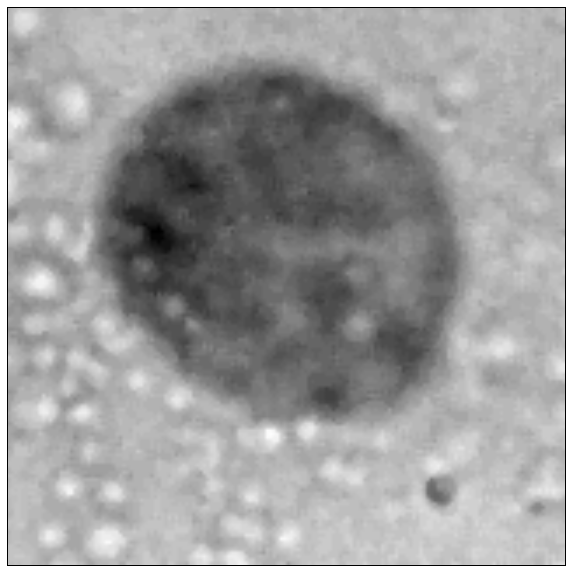
\includegraphics[width=1\linewidth]{Figures/Chapter3/fdim_0_1.png}
	\endminipage\hfill
	\minipage{0.4\textwidth}
	\centering	
	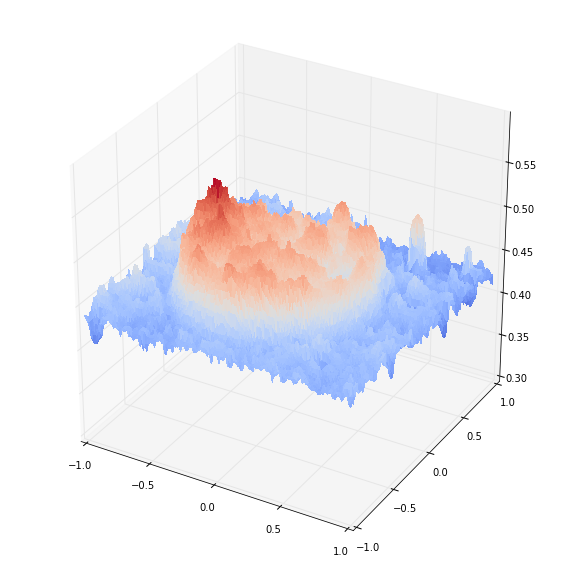
\includegraphics[width=1\linewidth]{Figures/Chapter3/fdim_0_2.png}
	\endminipage\hfill
	\minipage{0.3\textwidth}
	\centering	
	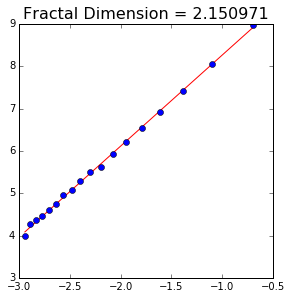
\includegraphics[width=1\linewidth]{Figures/Chapter3/fdim_0_3.png}
	\endminipage\hfill
	\endminipage\hfill
	\minipage{\textwidth}
	\minipage{0.3\textwidth}
	\centering
	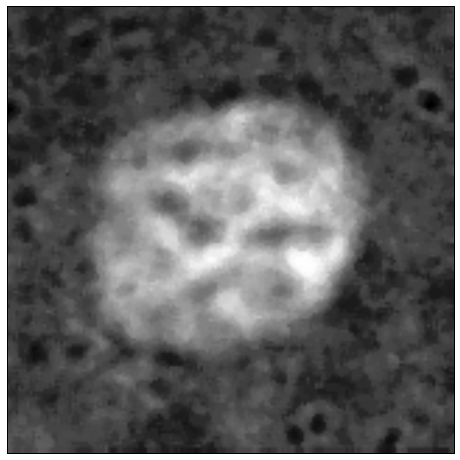
\includegraphics[width=1\linewidth]{Figures/Chapter3/fdim_1_1.png}
	\endminipage\hfill
	\minipage{0.4\textwidth}
	\centering		
	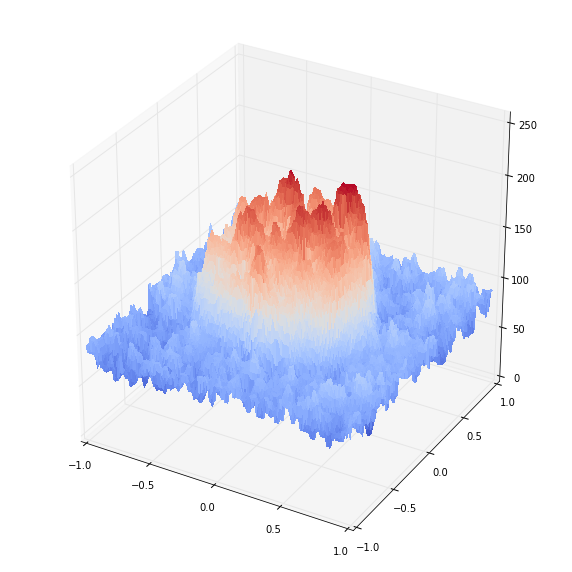
\includegraphics[width=1\linewidth]{Figures/Chapter3/fdim_1_2.png}
	\endminipage\hfill
	\minipage{0.3\textwidth}
	\centering	
	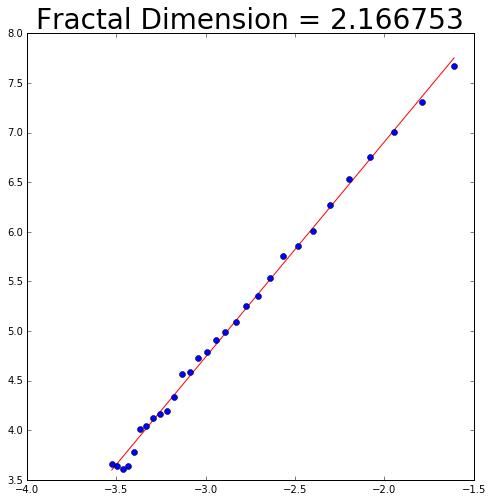
\includegraphics[width=1\linewidth]{Figures/Chapter3/fdim_1_3.png}
	\endminipage\hfill
	\endminipage\hfill
	
	\caption{Фрактальний аналіз зображень.}
	\label{fig:fdim}
\end{figure}

\section{Класифікація пацієнтів}

Слід помітити, що кожному пацієнту ставиться у відповідність набір (вибірка) фрак- тальних характеристик, розмір якої не є сталим. Отже, для порівняння набору характе- ристик різних пацієнтів, треба використовувати міру близькості між вибірками. 

\par
Оскільки міра близькості не є метрикою, вибір методів класифікації є дуже обмеженим. В цій роботі було використано найпростіший спосіб -- метод $k$ найближчих сусідів.

\subsection{Міра близькості та $p \textup{-статистика}$}

Через $H$ позначимо гіпотезу про рівность неперервних функцій розподілу $F_{G}(u)$ і $F_{G'}(u)$ генеральних сукупностей $G$ і $G'$ відповідно. Нехай вибірки $x = \left( x_1, x_2, \dots x_n \right) \in G$ і $x' = \left( x'_1, x'_2, \dots x'_m \right) \in G'$, $x_{(1)} \leq \dots \leq x_{(n)}$, $x_{(1)} \leq \dots \leq x_{(m)}$ -- порядкові статистики. Припустимо що $F_{G}(u) = F_{G'}(u)$. Позначимо через $A_{ij}^{(k)}, k = 1, 2, \dots m$ випадкова подія, яка полягає у тому, що $x'$ потрапляє в інтервал $\left( x_{(i)}, x_{(j)} \right)$, тобто $A_{ij}^{(k)} = \left\{ x'_k \in \left( x_{(i)}, x_{(j)} \right) \right\}$. Як відомо, ймовірність цієї події обчислюється за формулою:
$$P(A_{ij}^{(k)}) = P\left\{ x'_k \in \left( x_{(i)}, x_{(j)} \right) \right\} = p_{ij}^{(n)} = \frac{j-i}{n+1} = \frac{q}{n+1}, \quad q = j-i.$$

Покладемо 
$$ p_{ij}^{(1)} = \frac{ h_{ij}^{(n)}m + \frac{1}{2}g^2 - g\sqrt{h_{ij}^{(n)}(1-h)m + \frac{1}{4}g^2} }{ m+g^2 },$$
$$ p_{ij}^{(2)} = \frac{ h_{ij}^{(n)}m + \frac{1}{2}g^2 + g\sqrt{h_{ij}^{(n)}(1-h)m + \frac{1}{4}g^2} }{ m+g^2 },$$
де $h_{ij}^{(n)}$ -- частота події $A_{ij}^{(k)}$ в $m$ експериментів, величина $g = 3$.

Позначимо через $N$ кількість усіх довірчіх інтервалів $I_{ij}^{(n,m)} = \left( p_{ij}^{(1)}, p_{ij}^{(2)} \right)$ (тобто $N = {n(n-1)}/{2}$) і $L$ -- кількість інтервалів $I_{ij}^{(n,m)}$, які містять ймовірності $p_{ij}^{(n)}$. Покладемо $h^{(n,m)} = \rho(F^{*}, F^{*'}) = \rho(x, x') = {L}/{N}$. Оскільки $h^{(n,m)}$ -- частота випадкової події $B = \left\{ p_{ij}^{(n)} \in I_{ij}^{(n,m)} \right\}$, ймовірність якої дорівнює $p(B) = 1-\beta$, тоді, вважаючи що $h^{n,m}=h^{(n)}$, $m=N$ та $g=3$, отримаємо довірчий інтервал $I^{(n,m} = \left( p^{(1)}, p^{(2)}\right)$ для ймовірності $p(B)$. Статистика $h^{(n)}$ називається $p$-статистикою. Вона також є мірою близькості $\rho(x, x')$ між вибірками $x$ та $x'$ \parencite{bib:pstatistics}.


\subsection{Метод k найближчих сусiдiв. Кросвалідація.}

Використовуючи Метод k найближчих сусiдiв  для класифікації пацієнтів, необхідно зро- бити припущення коректності постулату про компактність:

\begin{conj}
	переважна бiльшiсть об’єктiв, що належать до одного класу, є ближчими один
	до одного, нiж до об’єктiв iншого класу, i лежать в областi з вiдносно простою межею.
\end{conj}

Суть цього методу для класифікації елементу $x$ полягає у тому, що з навчальної вибірки обираємо $k$ найближчих (у розумінні міри близькості) до $x$ елементів (характеристик пацієнтів) та відносимо $x$ до домінантного класу з цих $k$ елементів.

Для пошуку оптимального числа $k$, а також розміру навчальної вибірки $R$ використо- вують метод \textbf{кросвалідації}. Суть цього методу заключається у тому, що для кожного значення $k$ та $R$ випадковим чином підбирається набір даних для навчання.


\section{Результати та спостереження}

Вхідний набір даних для дослідження складається з знімків 6751 інтерфазних ядер букального епітелія, для кожного було зроблено 3 знімки мікроскопу: без фільтру, через жовтий фільтр та через пурпурного фільтру (отже всьго 20253 фотографії), взятого з 130 пацієнтів, з них 68 хворих раком, 29 здорових та 33 хворих іншою хворобою. 

Назвемо групу пацієнтів хворих на рак чи на фіброаденоматоз \enquote{позитивними}, а група здорових пацієнтів \enquote{негативними}. Тоді, за визначенню:

\begin{align*}
\begin{split}
\textup{чутливість} (sensitivity) = \frac{TP}{P}
\\
\textup{специфічність} (specificity) = \frac{TN}{N}
\end{split}
\end{align*}

де \(TP\) (true positive) -- кількість коректно класифікованих позитивних прикладів, \(TN\) (true negative) -- кількість коректно класифікованих негативних прикладів, \(P\) та \(N\) -- кількість позитивних та негативних прикладів у вибірці відповідно.

Нехай \(\Omega = R / N\), де \(R\) -- розмір навчальної вибірки, \(N\) -- розмір усієї вибірки.  Залежність середнього значення (після кросвалідації) чутливості від \(\Omega\) та кількості сусідів, аналі- зуючи червону компоненту зображень:
%-----------------------
%  RED CANCER
%-----------------------
\begin{center}
\begin{tabular}
{cc | c | c | c | c | c | c |}\cline{3-8}
& & \multicolumn{6}{ c| }{Кількість сусідів} \\ \cline{3-8}
& & 6 & 7 & 8 & 9 & 10 & 12 \\ \cline{1-8}

\multicolumn{1}{|c}{\multirow{5}{*}{
		\(\Omega\)
	}}
& \multicolumn{1}{ |c| }{0.5} & 
87.43\% & 81.42\% & 88.86\% & 83.71\% & 87.42\% & 85.43\% 

\\ \cline{2-8}
\multicolumn{1}{ |c  }{} & 
\multicolumn{1}{ |c| }{0.6} & 
83.93\% & 83.93\% & 86.78\% & 83.93\% & 87.14\% & 84.29\%

\\ \cline{2-8}
\multicolumn{1}{ |c  }{} & 
\multicolumn{1}{ |c| }{0.7} & 
85.23\% & 88.10\% & 89.05\% & 90.00\% & 87.62\% & 90.00\%

\\ \cline{2-8}
\multicolumn{1}{ |c  }{} & 
\multicolumn{1}{ |c| }{0.8} & 
87.14\% & 84.29\% & 90.00\% & 89.29\% & 86.43\% & 93.57\%

\\ \cline{2-8}
\multicolumn{1}{ |c  }{} & 
\multicolumn{1}{ |c| }{0.9} & 
82.86\% & 82.86\% & 85.71\% & 84.29\% & 91.42\% & 84.26\%

\\ \cline{1-8}
\end{tabular}
\end{center}



Залежність середнього значення (після кросвалідації) специфічності від \(\Omega\) та кількості сусідів, аналізуючи червону компоненту зображень:
%-----------------------
%  RED FIBRO
%-----------------------
\begin{center}
	\begin{tabular}
		{cc | c | c | c | c | c | c |}\cline{3-8}
		& & \multicolumn{6}{ c| }{Кількість сусідів} \\ \cline{3-8}
		& & 6 & 7 & 8 & 9 & 10 & 12 \\ \cline{1-8}
		
		\multicolumn{1}{|c}{\multirow{5}{*}{
				\(\Omega\)
		}}
		& \multicolumn{1}{ |c| }{0.5} & 
64.00\%	& 74.00\% & 63.33\% & 74.67\% & 62.00\% & 63.33\%
		
		\\ \cline{2-8}
		\multicolumn{1}{ |c  }{} & 
		\multicolumn{1}{ |c| }{0.6} & 
65.83\%	& 70.83\% & 65.33\% & 69.17\% & 64.17\% & 68.33\%
		
		\\ \cline{2-8}
		\multicolumn{1}{ |c  }{} & 
		\multicolumn{1}{ |c| }{0.7} & 
68.89\%	& 72.22\% & 58.89\% & 71.11\% & 73.33\% & 68.89\%
		
		\\ \cline{2-8}
		\multicolumn{1}{ |c  }{} & 
		\multicolumn{1}{ |c| }{0.8} & 
71.67\%	& 65.00\% & 68.33\% & 66.67\% & 73.33\% & 70.00\%
		
		\\ \cline{2-8}
		\multicolumn{1}{ |c  }{} & 
		\multicolumn{1}{ |c| }{0.9} & 
83.33\%	& 83.33\% & 53.33\% & 73.33\% & 66.67\% & 66.67\%
		
		\\ \cline{1-8}
	\end{tabular}
\end{center}


Залежність середнього значення (після кросвалідації) чутливості від \(\Omega\) та кількості сусідів, аналізуючи зелену компоненту зображень:
%-----------------------
%  GREEN CANCER
%-----------------------
\begin{center}
	\begin{tabular}
		{cc | c | c | c | c | c | c |}\cline{3-8}
		& & \multicolumn{6}{ c| }{Кількість сусідів} \\ \cline{3-8}
		& & 6 & 7 & 8 & 9 & 10 & 12 \\ \cline{1-8}
		
		\multicolumn{1}{|c}{\multirow{5}{*}{
				\(\Omega\)
		}}
		& \multicolumn{1}{ |c| }{0.5} & 
		90.86\% & 85.14\% & 	89.71\% & 	86.86\% & 	88.29\% & 	87.71\% 
		
		\\ \cline{2-8}
		\multicolumn{1}{ |c  }{} & 
		\multicolumn{1}{ |c| }{0.6} & 
87.50\% & 83.57\% & 	91.07\% & 	83.57\% & 	90.36\% & 	88.93\% 
		
		\\ \cline{2-8}
		\multicolumn{1}{ |c  }{} & 
		\multicolumn{1}{ |c| }{0.7} & 
81.90\% & 85.71\% & 	90.95\% & 	87.62\% & 	89.04\% & 	83.81\%
		
		\\ \cline{2-8}
		\multicolumn{1}{ |c  }{} & 
		\multicolumn{1}{ |c| }{0.8} & 
81.43\% & 83.57\% & 	88.57\% & 	80.00\% & 	89.29\% & 	91.43\% 
		
		\\ \cline{2-8}
		\multicolumn{1}{ |c  }{} & 
		\multicolumn{1}{ |c| }{0.9} & 
84.29\% & 87.14\% & 	88.57\% & 	87.14\% & 	85.71\% & 	82.86\% 
		
		\\ \cline{1-8}
	\end{tabular}
\end{center}

Залежність середнього значення (після кросвалідації) специфічності від \(\Omega\) та кількості сусідів, аналізуючи зелену компоненту зображень:
%-----------------------
%  GREEN FIBRO
%-----------------------
\begin{center}
	\begin{tabular}
		{cc | c | c | c | c | c | c |}\cline{3-8}
		& & \multicolumn{6}{ c| }{Кількість сусідів} \\ \cline{3-8}
		& & 6 & 7 & 8 & 9 & 10 & 12 \\ \cline{1-8}
		
		\multicolumn{1}{|c}{\multirow{5}{*}{
				\(\Omega\)
		}}
		& \multicolumn{1}{ |c| }{0.5} & 
63.33\% & 	71.33\% & 	67.33\% & 	67.33\% & 	66.67\% & 	60.67\% 
		
		\\ \cline{2-8}
		\multicolumn{1}{ |c  }{} & 
		\multicolumn{1}{ |c| }{0.6} & 
61.67\% & 	69.17\% & 	71.67\% & 	70.00\% & 	67.50\% & 	65.00\% 
		
		\\ \cline{2-8}
		\multicolumn{1}{ |c  }{} & 
		\multicolumn{1}{ |c| }{0.7} & 
71.11\% & 	70.00\% & 	61.11\% & 	77.78\% & 	66.67\% & 	70.00\%  
		
		\\ \cline{2-8}
		\multicolumn{1}{ |c  }{} & 
		\multicolumn{1}{ |c| }{0.8} & 
71.67\% & 	75.00\% & 	70.00\% & 	76.67\% & 	63.33\% & 	71.67\%  
		
		\\ \cline{2-8}
		\multicolumn{1}{ |c  }{} & 
		\multicolumn{1}{ |c| }{0.9} & 
60.00\% & 	63.33\% &  	70.00\% & 	76.67\% & 	73.33\% & 	70.00\%  
		
		\\ \cline{1-8}
	\end{tabular}
\end{center}

Залежність середнього значення (після кросвалідації) чутливості від \(\Omega\) та кількості сусідів, аналізуючи синю компоненту зображень:
%-----------------------
%  BLUE CANCER
%-----------------------
\begin{center}
	\begin{tabular}
		{cc | c | c | c | c | c | c |}\cline{3-8}
		& & \multicolumn{6}{ c| }{Кількість сусідів} \\ \cline{3-8}
		& & 6 & 7 & 8 & 9 & 10 & 12 \\ \cline{1-8}
		
		\multicolumn{1}{|c}{\multirow{5}{*}{
				\(\Omega\)
		}}
		& \multicolumn{1}{ |c| }{0.5} & 
88.86\% &	80.29\% &	86.86\% &	85.71\% &	89.71\% &	86.57\% 

		\\ \cline{2-8}
		\multicolumn{1}{ |c  }{} & 
		\multicolumn{1}{ |c| }{0.6} & 
84.29\% &	84.64\% &	87.14\% &	86.43\% &	90.36\% &	86.43\% 
		
		\\ \cline{2-8}
		\multicolumn{1}{ |c  }{} & 
		\multicolumn{1}{ |c| }{0.7} & 
88.57\% &	85.71\% &	91.90\% &	80.95\% &	90.00\% &	89.53\% 
		
		\\ \cline{2-8}
		\multicolumn{1}{ |c  }{} & 
		\multicolumn{1}{ |c| }{0.8} & 
84.29\% &	80.71\% &	89.29\% &	83.57\% &	90.71\% &	89.29\% 
		
		\\ \cline{2-8}
		\multicolumn{1}{ |c  }{} & 
		\multicolumn{1}{ |c| }{0.9} & 
82.86\% &	81.43\% &	91.43\% &	77.14\% &	92.80\% &	81.43\% 
		
		\\ \cline{1-8}
	\end{tabular}
\end{center}


Залежність середнього значення (після кросвалідації) специфічності від \(\Omega\) та кількості сусідів, аналізуючи синю компоненту зображень:
%-----------------------
%  BLUE CONTROL
%-----------------------
\begin{center}
	\begin{tabular}
		{cc | c | c | c | c | c | c |}\cline{3-8}
		& & \multicolumn{6}{ c| }{Кількість сусідів} \\ \cline{3-8}
		& & 6 & 7 & 8 & 9 & 10 & 12 \\ \cline{1-8}
		
		\multicolumn{1}{|c}{\multirow{5}{*}{
				\(\Omega\)
		}}
		& \multicolumn{1}{ |c| }{0.5} & 
62.67\% &	74.67\% &	66.67\% &	69.33\% &	61.33\% &	62.00\% 
		
		\\ \cline{2-8}
		\multicolumn{1}{ |c  }{} & 
		\multicolumn{1}{ |c| }{0.6} & 
66.67\% &	73.33\% &	65.00\% &	69.17\% &	64.17\% &	67.50\% 
		
		\\ \cline{2-8}
		\multicolumn{1}{ |c  }{} & 
		\multicolumn{1}{ |c| }{0.7} & 
60.00\% &	68.89\% &	62.22\% &	71.11\% &	61.11\% &	60.00\% 
		
		\\ \cline{2-8}
		\multicolumn{1}{ |c  }{} & 
		\multicolumn{1}{ |c| }{0.8} & 
55.00\% &	76.67\% &	65.00\% &	66.67\% &	61.67\% &	68.33\% 
		
		\\ \cline{2-8}
		\multicolumn{1}{ |c  }{} & 
		\multicolumn{1}{ |c| }{0.9} & 
76.67\% &	86.67\% &	70.00\% &	73.33\% &	70.00\% &	53.33\% 
		
		\\ \cline{1-8}
	\end{tabular}
\end{center}


Аналізуючи червону чи зелену компоненту зображень, можна отримати досить гарні результати чутливості та специфічності класифікатора (більші за 80\%). Нажаль, цей метод не дозволяє виявити відмінність між ядрами клітин пацієнтів з фіброаденоматозом та раком молочної залози.